\chapter{Introduction}

TODO: What is the big picture problem?

\section{Overview of Distributed Sensor Networks}
Distributed sensor networks (DSNs) consist of any number of sensors that collect and sense information about the physical environment around them. The sensors that make up these networks can either be homogeneous or heterogeneous. Distributed sensor networks are dynamic in that sensors can be added or removed from the network at any time. DSNs also increasingly include mobile sensors as well. With the onset of the Internet of Things (IoT), its easier than ever to build and deploy distributed sensor networks. Further, mobile devices, such as mobile phones, are seeing increased usage as intelligent sensing agents.

\subsection{DSN Data Collection Schemes}
Data can be collected from DSNs in various ways. Sensors can store data onboard to be collected manually or transmit data via a multitude of mediums (satellites, radio, laser, wired connections) using a slew of standards (TCP/IP, Zigbee, Bluetooth, custom, etc).

In some DSNs, data is routed between the sensors using various approaches and eventually makes its way to a sink or sinks. A sink is a data collection node. Cloud computing has become a prevalent choice for DSN sinks since they often provide the ability to provision resources as needed. Various approaches have been proposed that minimize and optimize communications between sensors within a DSN.

In other DSNs, sensor nodes have direct access to a sink, and instead of communicating with each other and passing messages among themselves, the nodes send their data directly to the sink. It's also possible for a DSN to take a hybrid approach and performs some communication within the network and some directly to the sink.

Not only are there various approaches to routing data, but there are also various approaches to deciding what kind of data to send (or acquire).

\subsection{DSN Detection Schemes}
On one extreme end, we have the send everything approach where each sensor sends its data to the sink all the time (or at least when it has the means to do). In this scenario, the sink is responsible for collection, cleaning, detection, and classification of signals and events within the data. This approach can be bandwidth and energy intensive, but provides the benefit of allowing more complete analysis to occur beyond the sink where more computational resources exist. This provides more accurate results and allows the sink to examine the results in aggregate with the rest of the DSN.

The other extreme is that sensors only send data when they have detected a signal of interest. In this scenario, sensors use onboard computing capabilities to filter their sensor stream and perform signal detection on the device. Only when the devices make a detection do they send the detection or data stream to a sink for further processing. This minimizes bandwidth but detection and classification of signals must occur with more constrained computing and energy environments. Further, the global state of the network can't be known without adding the complexity of sensor-to-sensor communication.

Often time a hybrid approach is taken where low fidelity feature extracted and sometimes aggregate data is sent from the sensors to the sink. The sink analyzes the low fidelity feature extracted stream to determine if raw data should be requested from the sensors. The act of requesting data from the sensors is called triggering. This approach is useful because we still gain bandwidth benefits and can easily gain an understanding of the global state of a network.

With all of these factors combined, management, collection, detection, localization, and analysis from distributed sensor networks is not a trivial task. DSNs can produce massive amounts of data. The emergence of IoT has increased the heterogeneity of sensors with multiple hardware configurations, variations of data APIs, and incomplete or bad sensor data. For these reasons, the data collected from distributed sensor networks under certain circumstances is considered Big Data.

\subsection{DSN Classification Schemes}
% TODO

\subsection{DSNs as Big Data}
Big Data is generally defined by the four V's; volume, velocity, variety, and value. These characteristics can be observed in many of the DSNs that exist and are being created today. % TODO more citations

That is, distributed sensor networks create a large volume of data due to the abundance of IoT and mobile devices that make up DSNs. As communication infrastructures improve and hardware becomes smaller, smarter and more energy efficient, sensors are able to send and transfer larger amounts of data. The ease of building and deploying sensors in DSNs means that more sensors can be produced much more cheaply allowing for more sensors to be used within a DSN, increasing coverage, but also increasing the volume of data.

Distributed sensor networks create a variety of data with different formats and data quality issues. Distributed sensor networks can produce data at high velocity. These characteristics of data produced from distributed sensor networks create a need for efficient architectures and specific algorithms designed for working with Big Data.

Further, sensor networks are often constrained in both computing power and available energy sources. This forces us to find comprises between data collection, onboard sensor processing, sensor communication, and network coordination.

\section{The Data Management and Analysis Problems}
All DSNs must decide how data is managed and analyzed. There are various approaches.

\section{Traditional Approaches to Data Management and Analysis}

\section{Laha}
I propose an abstract distributed sensor network framework, Laha, that adaptively optimizes triggering, collection, detection, classification, sensor device power requirements, and bandwidth. The Laha data model can be conceptualized as a multilevel pyramid (see fig. \ref{laha-abstract-overview}). Laha Actors act on the data model to move data upward through the levels and to apply optimizations downward through the levels.

The lowest level stores all recently received raw sensor data. This data expires and is automatically removed within a limited period of time (for example, 1 hour) unless the data is found to be interesting and is thus propagated upwards to the next level of the hierarchy.  Higher levels of the data hierarchy organize data in the same way, however each level adds context to the examined signal or signals. Context includes classifications, locality metrics, temporal metrics, or similarities to current or prior signals of interest. The highest level of the hierarchy, Phenomena, represents predictive capabilities of the sensor network which are then used to optimize and tune the lower levels.

A high level summary of the Laha abstract framework is provided as figure \ref{laha-abstract-overview}. The figure shows the levels and names of the hierarchy, a brief description of the functions of each level, and Laha's Actors and how they move data upwards (right hand side) and how they apply optimizations downwards (left hand side).

\begin{figure}
	\caption{Laha Conceptual Model Summary}
	\centering
	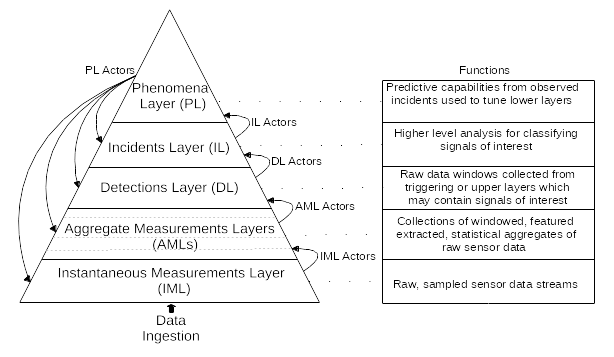
\includegraphics{figures/laha_abstract_overview.png}
	\label{laha-abstract-overview}
\end{figure}

The Laha framework aims to provide five useful benefits.
\begin{enumerate}
	\item Tiered management of Big Data where each tier has configurable time-to-live (TTL) requirements which provides a predicted upper bounds on bandwidth and storage requirements at the cost of potentially discarding important information.
	\item Automatically providing context to classified incidents based off of user and algorithmically tagged incidents. 
	\item Adaptive optimization of triggering within the network to decrease bandwidth and increase accuracy.
	\item Adaptive optimizations for detection and classification algorithms power by Laha's Phenomena.
	\item Building of a model of the underlying sensor field topology by observing how signals travel and are received across multiple devices.
\end{enumerate}

Laha will be evaluated by designing and implementing two Laha-compliant reference implementations, OPQMauka and Lokahi. Open Power Quality (OPQ) is a power quality (PQ) network consisting of custom hardware and distributed software services that detect distributed PQ signals such as voltage sags and swells, frequency sags and swells, transients, THD, and other known PQ issues. OPQMauka is a distributed, plugin based middleware component of OPQ that performs higher level analysis, data management, and optimizations of the OPQ services. Lokahi is a distributed infrasound network consisting of mobile iOS and Android devices and multiple cloud based software services whose purpose is to supplement the International Monitoring System (IMS) in detecting large infrasound signals.

The reference implementations will be designed and deployed to test sites at UH Manoa and at the Infrasound Laboratory in Kailua-Kona, Big Island during Q4 2018. 

Data collected from the PQ network will be validated against calibrated reference sensors that have already been installed at the power mains of a subset of buildings on campus during Q1 of 2019. The Office of Energy Management at UH Manoa has given us full access to live and historic PQ data collected at these reference sensors. OPQBoxes will be co-located and placed in buildings with the reference sensors so that we can validate that the triggering and raw data streams we receive from the OPQBoxes are in line with what the reference sensors are observing.

Data collected from the infrasound network will also be validated against industry standard calibrated BNK infrasound sensors. Further, signals in the infrasound network are known a priori since I am able to control the signals that are generated from our calibrated infrasound source, allowing further validation of received signals.

To evaluate the five benefits from Laha, several different approaches are taken depending on the Laha deployment and the benefit being evaluated. In the UH Manoa PQ deployment, we will co-locate sensors in our deployment and for each metric, one of the sensors will use Laha's optimizations and the other sensor will not. This will provide metrics that allows us to compare and contrast our optimization techniques within the OPQ network. 

In the Lokahi infrasound network, we will run a series of experiments where we can produce the same infrasound signals in each experiment and only change the tuning and optimizations that Laha applies to generate metrics for evaluation within the Laha network.

When evaluating the five proposed benefits of Laha, I will specifically look at the following metrics. 

For the tiered management of Big Data, I will measure the total amount of data saved and discarded at each level of the Laha data hierarchy while providing an upper bound of required storage for the given state of the network. I will also look at how the number of false positives and false negatives change when using Laha's tiered data management versus a ``store everything" approach. 

When evaluating automatically provided context of classified incident I will TODO.

In order to evaluate optimization of triggering, I will measure false positives and false negatives of triggered events. I will also evaluate if optimized triggering provides any benefits to overall bandwidth usage and sensor power requirements of the DSN.

To evaluate optimization of classification I will TODO.

Finally, to evaluate sensor field topology, we will collect TODO. 

% TODO provide name of industry standard OPQ sensors for validation

I expect to deploy reference implementations before the end of 2018 with validated data collection beginning and continuing through Q3 2019. I anticipate writing my dissertation along side the deployment and data collection process and to be finished in Q3 2019.

\section{Anticipated contributions of Laha}
Laha hopes to make the following four contributions to the areas of DSNs and specially optimization and management of DSNs.  First, the Laha design, a novel abstract distributed sensor network that provides five useful properties relating to data management, triggering, detection, classification, sensing field topology, predictive analytics, and self-optimization.

Second, an evaluation of the Laha abstract framework through the deployment of two Laha-compliant reference implementations, validated data collection, and several experiments that are used to either confirm or deny the benefits touted by Laha. 

Third, two Laha-compliant reference implementations, OPQ and Lokahi, which can be used to form DSNs for the collection of distributed power quality signals and the distributed collection of infrasound signals.

Fourth, a set of implications for modern distributed sensor networks as a result of the evaluation of Laha. That is, how does the confirmation of denial of Laha's benefits affect the field of modern DSNs moving forward?





